% !TeX root = defense_draft.tex
% ============================================================
% Defense draft v1 -- concrete content on the 21-slide
% storyboard. Audience assumption: committee members who have
% NOT read the thesis; every technical object gets one plain
% sentence before its name.
%
% Comment conventions:
%   SAY:        spoken narrative for the slide (not on slide)
%   WHY:        what the slide does for the argument
%   <<< ADAPT   path / content decision needed
%   <<< NUMBER  insert the exact figure from your results;
%               placeholders like [X %] are deliberate --
%               do NOT present invented numbers
%
% Build: latexmk -pdf defense_draft.tex
% ============================================================
\documentclass[11pt,aspectratio=169]{beamer}
\usetheme{default}
\usepackage[utf8]{inputenc}
\usepackage{amsmath}
\usepackage{amssymb}
\usepackage{graphicx}
\usepackage{tikz}
\usepackage{geometry}
\usetikzlibrary{positioning,calc,arrows.meta}

\setbeamertemplate{navigation symbols}{}
\setbeamertemplate{footline}[frame number]
\geometry{left=1cm}

\definecolor{Pone}{RGB}{83,74,183}    % P1 state space
\definecolor{Ptwo}{RGB}{216,90,48}    % P2 observation space
\definecolor{Pthree}{RGB}{29,158,117} % P3 physical space

\newcommand{\dd}{\mathrm d}
\DeclareMathOperator*{\argmax}{arg\,max}

\newcommand{\figplaceholder}[2][.7\linewidth]{%
  \fcolorbox{gray}{gray!10}{%
    \begin{minipage}[c][2.6cm][c]{#1}
      \centering\ttfamily\scriptsize #2
    \end{minipage}}}

% Staged synthesis schematic (see skeleton for stage meanings)
\newcommand{\synthstate}[1]{%
\ifnum#1>0 \tikzset{ponestyle/.style={draw=Pone, fill=Pone!12}}%
\else \tikzset{ponestyle/.style={draw=gray!70, text=gray}}\fi
\ifnum#1>1 \tikzset{ptwostyle/.style={draw=Ptwo, fill=Ptwo!12}}%
\else \tikzset{ptwostyle/.style={draw=gray!70, text=gray}}\fi
\ifnum#1>2 \tikzset{pthreestyle/.style={draw=Pthree,
                                        fill=Pthree!12}}%
\else \tikzset{pthreestyle/.style={draw=gray!70, text=gray}}\fi
\ifnum#1>3 \tikzset{corestyle/.style={fill=gray!12}}%
\else \tikzset{corestyle/.style={}}\fi
\begin{tikzpicture}[
    panel/.style={draw, rounded corners, align=center,
                  minimum width=4.2cm, minimum height=1.5cm},
    core/.style={draw=gray, dashed, rounded corners,
                 align=center, minimum width=4.6cm,
                 minimum height=1.7cm},
    leader/.style={gray, dotted, thick},
    rel/.style={->, thick},
    font=\small]
  \node[core, corestyle] (core) at (0,0)
    {\textbf{The mathematical toolkit}\\
     \scriptsize noise as probe $\cdot$ dimension as lens\\
     \scriptsize testbed: blocking \& WCBs};
  \node[panel, ponestyle] (p1) at (0,2.6)
    {\textbf{P1 $\cdot$ state space}\\
     \scriptsize perturb the system};
  \node[panel, ptwostyle] (p2) at (-4.6,-2.6)
    {\textbf{P2 $\cdot$ assimilation space}\\
     \scriptsize perturb the observations \\ \scriptsize and parametrization};
  \node[panel, pthreestyle] (p3) at (4.6,-2.6)
    {\textbf{P3 $\cdot$ physical space}\\
     \scriptsize perturb the air parcels};
  \draw[leader] (p1) -- (core);
  \draw[leader] (p2) -- (core);
  \draw[leader] (p3) -- (core);
  \ifnum#1>1
    \draw[rel] (p2.north) to[bend left=25]
      node[midway, left, align=right, font=\scriptsize]
      {spread $\perp$\\ unstable directions} (p1.west);
  \fi
  \ifnum#1>2
    \draw[rel] (p3.north) to[bend right=25]
      node[midway, right, align=left, font=\scriptsize]
      {dimension tracks\\ persistence} (p1.east);
  \fi
  \ifnum#1>3
    \draw[rel, <->] (p2.east) --
      node[midway, below, align=center, font=\scriptsize]
      {coherence controls \\ uncertainty in WCBs} (p3.west);
  \fi
\end{tikzpicture}}

% ============================================================
% fig_da_cycle.tex -- assimilation-cycle schematic
%
% Provides \dacyclefigure (a tikzpicture, no frame), sized for
% a .55\textwidth column at natural size -- do NOT wrap it in
% \resizebox, or the labels stop matching the body text.
%
% Overlays:
%   \dacycleoverlayson    9-step build (default)
%   \dacycleoverlaysoff   everything at once, single slide
% Set before calling \dacyclefigure.
%
% Label size: \renewcommand{\dacyclefont}{\small} etc.
%
% Include with:  % ============================================================
% fig_da_cycle.tex -- assimilation-cycle schematic
%
% Provides \dacyclefigure (a tikzpicture, no frame), sized for
% a .55\textwidth column at natural size -- do NOT wrap it in
% \resizebox, or the labels stop matching the body text.
%
% Overlays:
%   \dacycleoverlayson    9-step build (default)
%   \dacycleoverlaysoff   everything at once, single slide
% Set before calling \dacyclefigure.
%
% Label size: \renewcommand{\dacyclefont}{\small} etc.
%
% Include with:  % ============================================================
% fig_da_cycle.tex -- assimilation-cycle schematic
%
% Provides \dacyclefigure (a tikzpicture, no frame), sized for
% a .55\textwidth column at natural size -- do NOT wrap it in
% \resizebox, or the labels stop matching the body text.
%
% Overlays:
%   \dacycleoverlayson    9-step build (default)
%   \dacycleoverlaysoff   everything at once, single slide
% Set before calling \dacyclefigure.
%
% Label size: \renewcommand{\dacyclefont}{\small} etc.
%
% Include with:  \input{fig_da_cycle}   (NOT \include)
% Requires:      \usepackage{tikz}
%                \usetikzlibrary{arrows.meta}
% ============================================================

\providecommand{\dacycleoverlays}{1}
\providecommand{\dacycleoverlayson}{\renewcommand{\dacycleoverlays}{1}}
\providecommand{\dacycleoverlaysoff}{\renewcommand{\dacycleoverlays}{0}}
\providecommand{\dacyclefont}{\footnotesize}

% \dastep{overlay spec}{content}
\providecommand{\dastep}[2]{%
  \ifnum\dacycleoverlays=1 \only<#1>{#2}\else{#2}\fi}

\definecolor{fccol}{RGB}{220,50,40}
\definecolor{anacol}{RGB}{45,110,210}
\definecolor{obscol}{RGB}{20,120,90}

% \ebar{x}{y}{half-height}{colour}
\providecommand{\ebar}[4]{%
  \draw[#4, thick] (#1,{#2-#3}) -- (#1,{#2+#3});
  \draw[#4, thick] ({#1-0.09},{#2-#3}) -- ({#1+0.09},{#2-#3});
  \draw[#4, thick] ({#1-0.09},{#2+#3}) -- ({#1+0.09},{#2+#3});}

% \anastep{x}{y}{half-height}
\providecommand{\anastep}[3]{%
  \ebar{#1}{#2}{#3}{anacol}
  \fill[anacol] ({#1-0.085},{#2-0.045})
  rectangle ({#1+0.085},{#2+0.045});}

\providecommand{\dacyclefigure}{%
  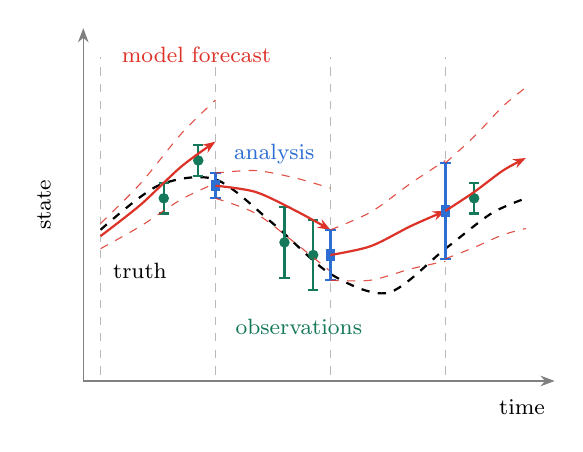
\begin{tikzpicture}[x=0.73cm, y=1.60cm, font=\dacyclefont,
    fcline/.style={fccol, thick, -{Stealth[length=1.6mm]}},
    fcband/.style={fccol, thin, dashed, opacity=.85}]

    \draw[-{Stealth[length=1.8mm]}, gray]
    (1.7,1.15) -- (9.9,1.15);
    \node[anchor=north east] at (9.9,1.08) {time};
    \draw[-{Stealth[length=1.8mm]}, gray]
    (1.7,1.15) -- (1.7,3.95);
    \node[rotate=90, anchor=south] at (1.30,2.55) {state};

    % --- 1: truth + assimilation windows ---
    \foreach \t in {2,4,6,8}{
        \draw[gray!55, dashed] (\t,1.2) -- (\t,3.72);
      }
    \draw[black, thick, dashed] plot[smooth]
    coordinates {(2,2.35) (3,2.70) (4,2.75) (5,2.40)
        (6,2.00) (7,1.85) (8,2.20) (8.8,2.48)
        (9.4,2.60)};
    \node[anchor=north west] at (2.05,2.16) {truth};

    % --- 2: observations ---
    \dastep{2-}{%
      \foreach \x/\y/\e in {3.1/2.60/0.12, 3.7/2.90/0.12,
          5.2/2.25/0.28, 5.7/2.15/0.28,
          8.5/2.60/0.12}{
          \ebar{\x}{\y}{\e}{obscol}
          \fill[obscol] (\x,\y) circle (1.9pt);
        }
      \node[obscol, anchor=north] at (5.45,1.72)
      {observations};
    }

    % --- 3: forecast, window 1 ---
    \dastep{3-}{%
      \draw[fcline] plot[smooth] coordinates
        {(2,2.30) (2.7,2.55) (3.4,2.85) (4,3.05)};
      \draw[fcband] plot[smooth] coordinates
        {(2,2.40) (2.7,2.72) (3.4,3.11) (4,3.38)};
      \draw[fcband] plot[smooth] coordinates
        {(2,2.20) (2.7,2.38) (3.4,2.59) (4,2.72)};
      \node[fccol, anchor=south west] at (2.2,3.60)
      {model forecast};
    }

    % --- 4: analysis, end of window 1 ---
    \dastep{4-}{%
      \anastep{4}{2.70}{0.10}
      \node[anacol, anchor=south west] at (4.15,2.80)
      {analysis};
    }

    % --- 5: forecast, window 2 ---
    \dastep{5-}{%
      \draw[fcline] plot[smooth] coordinates
        {(4,2.70) (4.7,2.65) (5.4,2.50) (6,2.35)};
      \draw[fcband] plot[smooth] coordinates
        {(4,2.80) (4.7,2.82) (5.4,2.76) (6,2.68)};
      \draw[fcband] plot[smooth] coordinates
        {(4,2.60) (4.7,2.48) (5.4,2.24) (6,2.02)};
    }

    % --- 6: analysis, end of window 2 ---
    \dastep{6-}{\anastep{6}{2.15}{0.20}}

    % --- 7: forecast, window 3 ---
    \dastep{7-}{%
      \draw[fcline] plot[smooth] coordinates
        {(6,2.15) (6.7,2.22) (7.4,2.38) (8,2.50)};
      \draw[fcband] plot[smooth] coordinates
        {(6,2.35) (6.7,2.49) (7.4,2.72) (8,2.90)};
      \draw[fcband] plot[smooth] coordinates
        {(6,1.95) (6.7,1.95) (7.4,2.04) (8,2.10)};
    }

    % --- 8: analysis, end of window 3 ---
    \dastep{8-}{\anastep{8}{2.50}{0.38}}

    % --- 9: forecast from the uncertain analysis ---
    \dastep{9-}{%
      \draw[fcline] plot[smooth] coordinates
        {(8,2.50) (8.5,2.65) (9.0,2.82) (9.4,2.92)};
      \draw[fcband] plot[smooth] coordinates
        {(8,2.88) (8.5,3.09) (9.0,3.33) (9.4,3.48)};
      \draw[fcband] plot[smooth] coordinates
        {(8,2.12) (8.5,2.21) (9.0,2.31) (9.4,2.36)};
    }
  \end{tikzpicture}}   (NOT \include)
% Requires:      \usepackage{tikz}
%                \usetikzlibrary{arrows.meta}
% ============================================================

\providecommand{\dacycleoverlays}{1}
\providecommand{\dacycleoverlayson}{\renewcommand{\dacycleoverlays}{1}}
\providecommand{\dacycleoverlaysoff}{\renewcommand{\dacycleoverlays}{0}}
\providecommand{\dacyclefont}{\footnotesize}

% \dastep{overlay spec}{content}
\providecommand{\dastep}[2]{%
  \ifnum\dacycleoverlays=1 \only<#1>{#2}\else{#2}\fi}

\definecolor{fccol}{RGB}{220,50,40}
\definecolor{anacol}{RGB}{45,110,210}
\definecolor{obscol}{RGB}{20,120,90}

% \ebar{x}{y}{half-height}{colour}
\providecommand{\ebar}[4]{%
  \draw[#4, thick] (#1,{#2-#3}) -- (#1,{#2+#3});
  \draw[#4, thick] ({#1-0.09},{#2-#3}) -- ({#1+0.09},{#2-#3});
  \draw[#4, thick] ({#1-0.09},{#2+#3}) -- ({#1+0.09},{#2+#3});}

% \anastep{x}{y}{half-height}
\providecommand{\anastep}[3]{%
  \ebar{#1}{#2}{#3}{anacol}
  \fill[anacol] ({#1-0.085},{#2-0.045})
  rectangle ({#1+0.085},{#2+0.045});}

\providecommand{\dacyclefigure}{%
  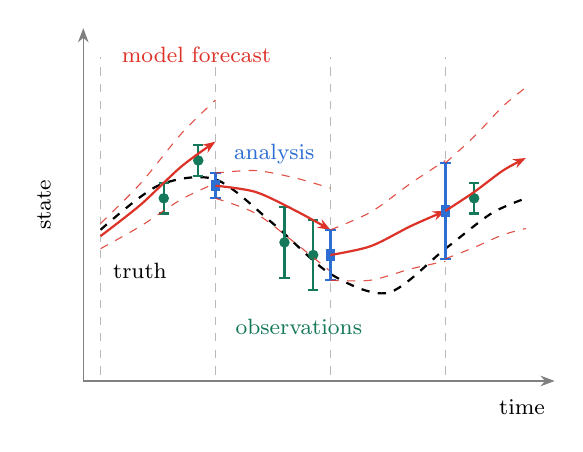
\begin{tikzpicture}[x=0.73cm, y=1.60cm, font=\dacyclefont,
    fcline/.style={fccol, thick, -{Stealth[length=1.6mm]}},
    fcband/.style={fccol, thin, dashed, opacity=.85}]

    \draw[-{Stealth[length=1.8mm]}, gray]
    (1.7,1.15) -- (9.9,1.15);
    \node[anchor=north east] at (9.9,1.08) {time};
    \draw[-{Stealth[length=1.8mm]}, gray]
    (1.7,1.15) -- (1.7,3.95);
    \node[rotate=90, anchor=south] at (1.30,2.55) {state};

    % --- 1: truth + assimilation windows ---
    \foreach \t in {2,4,6,8}{
        \draw[gray!55, dashed] (\t,1.2) -- (\t,3.72);
      }
    \draw[black, thick, dashed] plot[smooth]
    coordinates {(2,2.35) (3,2.70) (4,2.75) (5,2.40)
        (6,2.00) (7,1.85) (8,2.20) (8.8,2.48)
        (9.4,2.60)};
    \node[anchor=north west] at (2.05,2.16) {truth};

    % --- 2: observations ---
    \dastep{2-}{%
      \foreach \x/\y/\e in {3.1/2.60/0.12, 3.7/2.90/0.12,
          5.2/2.25/0.28, 5.7/2.15/0.28,
          8.5/2.60/0.12}{
          \ebar{\x}{\y}{\e}{obscol}
          \fill[obscol] (\x,\y) circle (1.9pt);
        }
      \node[obscol, anchor=north] at (5.45,1.72)
      {observations};
    }

    % --- 3: forecast, window 1 ---
    \dastep{3-}{%
      \draw[fcline] plot[smooth] coordinates
        {(2,2.30) (2.7,2.55) (3.4,2.85) (4,3.05)};
      \draw[fcband] plot[smooth] coordinates
        {(2,2.40) (2.7,2.72) (3.4,3.11) (4,3.38)};
      \draw[fcband] plot[smooth] coordinates
        {(2,2.20) (2.7,2.38) (3.4,2.59) (4,2.72)};
      \node[fccol, anchor=south west] at (2.2,3.60)
      {model forecast};
    }

    % --- 4: analysis, end of window 1 ---
    \dastep{4-}{%
      \anastep{4}{2.70}{0.10}
      \node[anacol, anchor=south west] at (4.15,2.80)
      {analysis};
    }

    % --- 5: forecast, window 2 ---
    \dastep{5-}{%
      \draw[fcline] plot[smooth] coordinates
        {(4,2.70) (4.7,2.65) (5.4,2.50) (6,2.35)};
      \draw[fcband] plot[smooth] coordinates
        {(4,2.80) (4.7,2.82) (5.4,2.76) (6,2.68)};
      \draw[fcband] plot[smooth] coordinates
        {(4,2.60) (4.7,2.48) (5.4,2.24) (6,2.02)};
    }

    % --- 6: analysis, end of window 2 ---
    \dastep{6-}{\anastep{6}{2.15}{0.20}}

    % --- 7: forecast, window 3 ---
    \dastep{7-}{%
      \draw[fcline] plot[smooth] coordinates
        {(6,2.15) (6.7,2.22) (7.4,2.38) (8,2.50)};
      \draw[fcband] plot[smooth] coordinates
        {(6,2.35) (6.7,2.49) (7.4,2.72) (8,2.90)};
      \draw[fcband] plot[smooth] coordinates
        {(6,1.95) (6.7,1.95) (7.4,2.04) (8,2.10)};
    }

    % --- 8: analysis, end of window 3 ---
    \dastep{8-}{\anastep{8}{2.50}{0.38}}

    % --- 9: forecast from the uncertain analysis ---
    \dastep{9-}{%
      \draw[fcline] plot[smooth] coordinates
        {(8,2.50) (8.5,2.65) (9.0,2.82) (9.4,2.92)};
      \draw[fcband] plot[smooth] coordinates
        {(8,2.88) (8.5,3.09) (9.0,3.33) (9.4,3.48)};
      \draw[fcband] plot[smooth] coordinates
        {(8,2.12) (8.5,2.21) (9.0,2.31) (9.4,2.36)};
    }
  \end{tikzpicture}}   (NOT \include)
% Requires:      \usepackage{tikz}
%                \usetikzlibrary{arrows.meta}
% ============================================================

\providecommand{\dacycleoverlays}{1}
\providecommand{\dacycleoverlayson}{\renewcommand{\dacycleoverlays}{1}}
\providecommand{\dacycleoverlaysoff}{\renewcommand{\dacycleoverlays}{0}}
\providecommand{\dacyclefont}{\footnotesize}

% \dastep{overlay spec}{content}
\providecommand{\dastep}[2]{%
  \ifnum\dacycleoverlays=1 \only<#1>{#2}\else{#2}\fi}

\definecolor{fccol}{RGB}{220,50,40}
\definecolor{anacol}{RGB}{45,110,210}
\definecolor{obscol}{RGB}{20,120,90}

% \ebar{x}{y}{half-height}{colour}
\providecommand{\ebar}[4]{%
  \draw[#4, thick] (#1,{#2-#3}) -- (#1,{#2+#3});
  \draw[#4, thick] ({#1-0.09},{#2-#3}) -- ({#1+0.09},{#2-#3});
  \draw[#4, thick] ({#1-0.09},{#2+#3}) -- ({#1+0.09},{#2+#3});}

% \anastep{x}{y}{half-height}
\providecommand{\anastep}[3]{%
  \ebar{#1}{#2}{#3}{anacol}
  \fill[anacol] ({#1-0.085},{#2-0.045})
  rectangle ({#1+0.085},{#2+0.045});}

\providecommand{\dacyclefigure}{%
  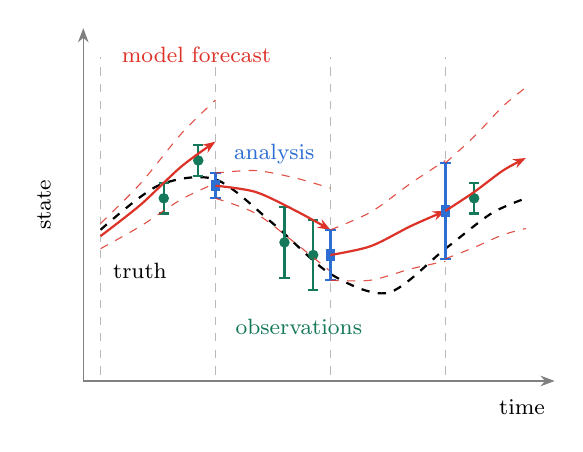
\begin{tikzpicture}[x=0.73cm, y=1.60cm, font=\dacyclefont,
    fcline/.style={fccol, thick, -{Stealth[length=1.6mm]}},
    fcband/.style={fccol, thin, dashed, opacity=.85}]

    \draw[-{Stealth[length=1.8mm]}, gray]
    (1.7,1.15) -- (9.9,1.15);
    \node[anchor=north east] at (9.9,1.08) {time};
    \draw[-{Stealth[length=1.8mm]}, gray]
    (1.7,1.15) -- (1.7,3.95);
    \node[rotate=90, anchor=south] at (1.30,2.55) {state};

    % --- 1: truth + assimilation windows ---
    \foreach \t in {2,4,6,8}{
        \draw[gray!55, dashed] (\t,1.2) -- (\t,3.72);
      }
    \draw[black, thick, dashed] plot[smooth]
    coordinates {(2,2.35) (3,2.70) (4,2.75) (5,2.40)
        (6,2.00) (7,1.85) (8,2.20) (8.8,2.48)
        (9.4,2.60)};
    \node[anchor=north west] at (2.05,2.16) {truth};

    % --- 2: observations ---
    \dastep{2-}{%
      \foreach \x/\y/\e in {3.1/2.60/0.12, 3.7/2.90/0.12,
          5.2/2.25/0.28, 5.7/2.15/0.28,
          8.5/2.60/0.12}{
          \ebar{\x}{\y}{\e}{obscol}
          \fill[obscol] (\x,\y) circle (1.9pt);
        }
      \node[obscol, anchor=north] at (5.45,1.72)
      {observations};
    }

    % --- 3: forecast, window 1 ---
    \dastep{3-}{%
      \draw[fcline] plot[smooth] coordinates
        {(2,2.30) (2.7,2.55) (3.4,2.85) (4,3.05)};
      \draw[fcband] plot[smooth] coordinates
        {(2,2.40) (2.7,2.72) (3.4,3.11) (4,3.38)};
      \draw[fcband] plot[smooth] coordinates
        {(2,2.20) (2.7,2.38) (3.4,2.59) (4,2.72)};
      \node[fccol, anchor=south west] at (2.2,3.60)
      {model forecast};
    }

    % --- 4: analysis, end of window 1 ---
    \dastep{4-}{%
      \anastep{4}{2.70}{0.10}
      \node[anacol, anchor=south west] at (4.15,2.80)
      {analysis};
    }

    % --- 5: forecast, window 2 ---
    \dastep{5-}{%
      \draw[fcline] plot[smooth] coordinates
        {(4,2.70) (4.7,2.65) (5.4,2.50) (6,2.35)};
      \draw[fcband] plot[smooth] coordinates
        {(4,2.80) (4.7,2.82) (5.4,2.76) (6,2.68)};
      \draw[fcband] plot[smooth] coordinates
        {(4,2.60) (4.7,2.48) (5.4,2.24) (6,2.02)};
    }

    % --- 6: analysis, end of window 2 ---
    \dastep{6-}{\anastep{6}{2.15}{0.20}}

    % --- 7: forecast, window 3 ---
    \dastep{7-}{%
      \draw[fcline] plot[smooth] coordinates
        {(6,2.15) (6.7,2.22) (7.4,2.38) (8,2.50)};
      \draw[fcband] plot[smooth] coordinates
        {(6,2.35) (6.7,2.49) (7.4,2.72) (8,2.90)};
      \draw[fcband] plot[smooth] coordinates
        {(6,1.95) (6.7,1.95) (7.4,2.04) (8,2.10)};
    }

    % --- 8: analysis, end of window 3 ---
    \dastep{8-}{\anastep{8}{2.50}{0.38}}

    % --- 9: forecast from the uncertain analysis ---
    \dastep{9-}{%
      \draw[fcline] plot[smooth] coordinates
        {(8,2.50) (8.5,2.65) (9.0,2.82) (9.4,2.92)};
      \draw[fcband] plot[smooth] coordinates
        {(8,2.88) (8.5,3.09) (9.0,3.33) (9.4,3.48)};
      \draw[fcband] plot[smooth] coordinates
        {(8,2.12) (8.5,2.21) (9.0,2.31) (9.4,2.36)};
    }
  \end{tikzpicture}}   % in the preamble

% ============================================================
% fig_coherent_sets.tex -- coherent vs. incoherent set under
% perturbation.  Columns are time, rows are with/without the
% perturbed ensemble.  Revealed in four steps, clockwise:
%   1 top-left      t0, two sets, unperturbed
%   2 top-right     t1, advected: one compact, one filamented
%   3 bottom-right  t1, with the perturbed ensemble
%   4 bottom-left   t0, with the perturbed ensemble
%
% Provides \coherentsetsfigure (a tikzpicture, no frame).
%
% Overlays:
%   \csoverlayson    four-step build (default)
%   \csoverlaysoff   all four panels at once
% Set before calling \coherentsetsfigure.
%
% NB: panels are written in reveal order so the dot fields stay
% pixel-identical from one overlay to the next.
%
% Include with:  \input{fig_coherent_sets}   (NOT \include)
% Requires:      \usepackage{tikz}
% ============================================================

\providecommand{\csoverlays}{1}
\providecommand{\csoverlayson}{\renewcommand{\csoverlays}{1}}
\providecommand{\csoverlaysoff}{\renewcommand{\csoverlays}{0}}

% \csstep{overlay spec}{content}
\providecommand{\csstep}[2]{%
  \ifnum\csoverlays=1 \only<#1>{#2}\else{#2}\fi}

\definecolor{dotred}{RGB}{205,15,15}
\definecolor{blobgray}{RGB}{168,168,168}

\providecommand{\panelframe}{%
  \draw[gray!55, line width=0.4pt] (0,0) rectangle (5,2.5);}

% \cluster{cx}{cy}{radius}{count}
\providecommand{\cluster}[4]{%
  \begin{scope}[shift={(#1,#2)}]
    \foreach \i in {1,...,#4}{
      \pgfmathsetmacro{\a}{360*rnd}
      \pgfmathsetmacro{\d}{#3*sqrt(rnd)}
      \fill[dotred] (\a:\d) circle (0.55pt);
    }
  \end{scope}}

% spiral radius, in cm, as a function of angle in degrees
\providecommand{\spiralr}[1]{0.601+0.000978*#1}

\providecommand{\coherentsetsfigure}{%
  % seed reset on every overlay so the dots never jitter
  \pgfmathsetseed{11}%
  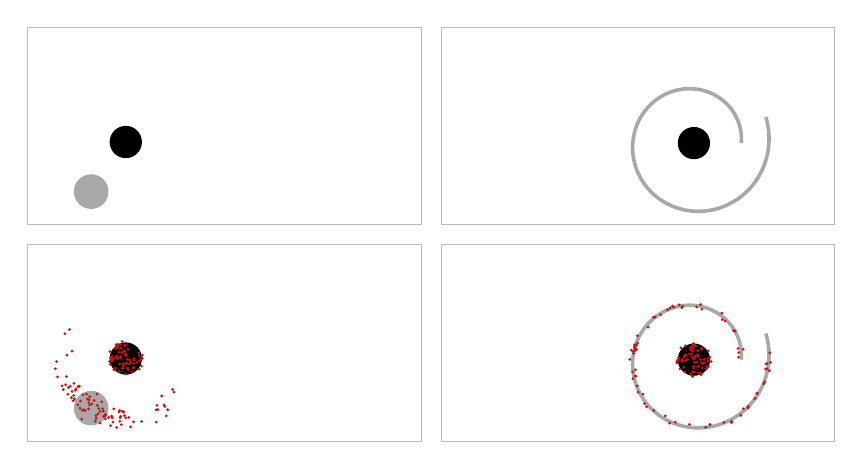
\begin{tikzpicture}
    % fixed bounding box: panels appear without shifting layout
    \path[use as bounding box] (0,0) rectangle (10.25,5.25);

    % ---------- 1: top-left -- t0, unperturbed ----------
    \csstep{4-}{%
      \begin{scope}[shift={(0,2.75)}]
        \panelframe
        \fill[black]    (1.246,1.048) circle (0.205);
        \fill[blobgray] (0.806,0.418) circle (0.220);
      \end{scope}}

    % ---------- 2: top-right -- t1, unperturbed ----------
    \csstep{5-}{%
      \begin{scope}[shift={(5.25,2.75)}]
        \panelframe
        \begin{scope}[shift={(3.211,1.034)}]
          \draw[blobgray, line width=1.3pt, smooth]
            plot[domain=0:380, samples=140, variable=\t]
            ({\t}:{\spiralr{\t}});
        \end{scope}
        \fill[black] (3.211,1.034) circle (0.205);
      \end{scope}}

    % ---------- 3: bottom-right -- t1, with ensemble ----------
    \csstep{6-}{%
      \begin{scope}[shift={(5.25,0)}]
        \panelframe
        \begin{scope}[shift={(3.211,1.034)}]
          \draw[blobgray, line width=1.3pt, smooth]
            plot[domain=0:380, samples=140, variable=\t]
            ({\t}:{\spiralr{\t}});
          \foreach \i in {1,...,72}{
            \pgfmathsetmacro{\t}{380*rnd}
            \pgfmathsetmacro{\r}{\spiralr{\t}+0.038*rand}
            \fill[dotred] ({\t}:{\r}) circle (0.55pt);
          }
        \end{scope}
        \fill[black] (3.211,1.034) circle (0.205);
        \cluster{3.211}{1.034}{0.225}{70}
      \end{scope}}

    % ---------- 4: bottom-left -- t0, with ensemble ----------
    \csstep{7-}{%
      \begin{scope}[shift={(0,0)}]
        \panelframe
        \fill[black]    (1.246,1.048) circle (0.205);
        \fill[blobgray] (0.806,0.418) circle (0.220);
        % coherent set: ensemble stays on the blob
        \cluster{1.246}{1.048}{0.225}{70}
        % incoherent set: ensemble strung out along the emerging
        % filament -- an arc about the coherent set, the first
        % part of the spiral fully wound in the top-right panel
        \begin{scope}[shift={(1.246,1.048)}]
          \foreach \i in {1,...,45}{
            \pgfmathsetmacro{\t}{205+70*rnd}
            \pgfmathsetmacro{\r}{0.777+0.115*rand}
            \fill[dotred] (\t:\r) circle (0.55pt);
          }
          \foreach \i in {1,...,33}{
            \pgfmathsetmacro{\t}{150+180*rnd}
            \pgfmathsetmacro{\r}{0.777+0.130*rand}
            \fill[dotred] (\t:\r) circle (0.55pt);
          }
        \end{scope}
        \cluster{0.806}{0.418}{0.20}{12}
      \end{scope}}
  \end{tikzpicture}}

\author{Henry Schoeller}
\title{Atmospheric Blocking and Warm Conveyor Belts:
       Mathematical Perspectives}
\date{September 14, 2026} % <<< ADAPT: exact defense date

\begin{document}

% ============================================================
% OPENING (~3 min)
% ============================================================

% WHY: plant the one sentence the whole defense hangs on.
% SAY: "Welcome to the presentation of my doctoral thesis with the title 
% `Atmospheric Blocking and Warm Conveyor Belts: Mathematical Perspectives'.
% In one sentence: this thesis
%   explores the coupling of blocking and warm conveyor belts by developing
%   and applying a mathematical toolkit whose applicability transcends the 
%   specific system."
\begin{frame}
  \titlepage
  \vspace{-1.0cm}
  \begin{center}
    \includegraphics[width=.25\textwidth]{../fu-logo-250708-CMYK-p.pdf} \hspace{1cm} \includegraphics[width=.25\textwidth]{../CRC1114_Logos/LOGO_GRUEN_RGB_CRC.pdf}
  \end{center}
\end{frame}

% WHY: why we should care about blocks.
% SAY: "But to illustrate why investigating blocks is important, I want to call
%   back into memory an illustrative example of an impactful atmospheric
%   blocking event---the heat wave Europe experienced this June."
% \begin{frame}{June 2026 heat wave}
%   \centering
%   \hspace*{-1cm}
%   \only<1>{\includegraphics[scale=1]
%     {../../../wp22a/figs/build_1_temp.pdf}}%
%   \only<2>{\includegraphics[scale=1]
%     {../../../wp22a/figs/build_2_z.pdf}}%
%   \only<3>{\includegraphics[scale=1]
%     {../../../wp22a/figs/build_3_mslp.pdf}}%
%   \only<4>{\includegraphics[scale=1]
%     {../../../wp22a/figs/build_4_satellite.pdf}}%
% \end{frame}

% WHY: generalize from the June 2026 case to the phenomena
%   themselves; introduce WCBs as a first-class protagonist,
%   not just a mechanism note on blocks.
% SAY: "But why should we care about blockings and warm conveyor belts and 
% why are does their investigation call for advanced mathematical methods?
% A blocking is a high-impact, persistent weather regime crucially shaping
% the mid-latitude circulation while still posing significant challenges
% for both weather and climate models. This is likely due to the vast range of 
% scales and physical processes exerting influence on their dynamics and 
% morphology. 
% Warm conveyor belts are just as
%   consequential in their own right: they redistribute heat
%   and moisture on a hemispheric scale and play a crucial role in  
%   forecast-uncertainty growth. These features lead to them being considered
% one of the prime conduits of diabatic influence on the large-scale flow. 
% And critically
%   for this thesis, the two are not independent -- blocking
%   and WCBs have been shown to interact strongly, as depicted in this
% schematic: WCBs caused by upstream low-pressure systems lead to negative 
% PV anomalies in upper levels enforcing a blocking systems strength as well as
% their stationarity, because the anomaly is enforced at their upstream flank.
% That coupling is the
%   system this thesis is built around. But rather than simply reiterating each
% of the 
% physical insights obtained in the three papers the thesis is built on,
% I want to structure this presentation by focussing on the commonalities of
% the mathematical methods developed and applied."
\begin{frame}{Blocking and warm conveyor belts}
  \begin{columns}
    \begin{column}{.4\textwidth}
      \textbf{Blocking}
      \begin{itemize}
        \item High-impact, persistent weather regime \pause
        \item Challenging for models \pause
        \item Range of scales and processes \pause
      \end{itemize}
      \bigskip
      \textbf{Warm conveyor belts}
      \begin{itemize}
        \item Synoptic features responsible for heat and moisture transport \pause
        \item Amplifiers of forecast uncertainty \pause
        \item Diabatic influence on the large-scale flow \pause
      \end{itemize}
    \end{column}
    \begin{column}{.6\textwidth}
      \centering
      \includegraphics[scale=.35,  trim={4.5cm 8cm 6cm 0cm}, clip]{../Thesis/fig/Intro/f01.pdf}
      {\tiny Steinfeld (2019)}
    \end{column}
  \end{columns}
\end{frame}


% WHY: roadmap; promises the synthesis without spoiling it.
% SAY: "The thesis asks three questions about this system, and
%   -- this is the point -- answers all three with the same
%   operation: perturb something and watch the response while consistently
% reflecting on the associated dimensions -- dynamical or physical. The three
% papers are ordered from most abstract to most concrete. Paper
%   one perturbs the trajectory of the system in state space.
%   Paper two analyzes perturbation to the observations and parametrizations
% in assimilation space. And paper three perturbs
%   air parcels themselves in physical space. By
%   the end of the presentation, this picture will be filled in."
\begin{frame}{}
  \centering
  \synthstate{0}
\end{frame}

% ============================================================
% PAPER 1 -- STATE SPACE (~5 min)
% ============================================================

% WHY: establish the state-space picture before any dynamics.
%   Build: (1) deterministic attractor alone, (2) fixed points
%   marked via the right panel, (3) right panel becomes the
%   stochastic attractor -- deterministic vs stochastic side by
%   side, motivating "what does noise do to these regimes?"
% SAY (1): "As mentioned before, the first paper adopts an abstract dynamical 
% systems perspective by considering the Charney-DeVore-model, whose attractor
% is shown here in principle component space. The system mainly travels on
% these highly populated orbits as indicated by the logarithmic density scale.
% It irregularly collapses to this one-dimensional submanifold before
% transitioning to quasi-periodic chaotic oscillations before collapsing again.
% SAY (2): "The dynamics are critically shaped by the two unstable fixed points indicated
% here by the red and black crosses, which happen to correspond -- not
% coincidentially -- to a zonal and blocked flow state respectively.
% In models of the atmosphere small random perturbations or "noise" is
% commonly used to represent unresolved
% processes and uncertainties, so a possible interpretation of this noise
% is that we treat it as a stand-in for moist effects; the effects of WCBs
% in particular."
% SAY (3): "What happens when we add noise of strength sigma to the system at
% hand and rerun the simulation? 
% As expected, the noise smears out the detailed structure of the attractor
%  -- but it also allows the system to explore regions of the state space that
% were previously inaccessible and the general regime structure survives. 
% For such a low-dimensional system, resimultaion for different noise levels
% is feasible, but for other systems, this may not be the case and one may not
% even have access to the governing equations."
\begin{frame}{Charney--DeVore: a paradigm for regime dynamics}
  \centering
  \hspace*{-1cm}
  \begin{tikzpicture}[scale=16/15]
    % --- LEFT panel: deterministic attractor, all states ---
    \node[anchor=center,inner sep=0] (left)
    {\includegraphics[scale=.75]
      {fig/HistPlotsPC_nolabel.pdf}};

    % --- RIGHT panel: fixed points (2) then stochastic (3) ---
    \only<2>{
      \node[anchor=west,inner sep=0,right=6pt of left] (right)
      {\includegraphics[scale=.75]
        {fig/fixed_points_nolabel.pdf}};
    }

    \only<3>{
    \node[anchor=west,inner sep=0,right=100pt of left] (right)
    {\includegraphics[scale=.75]
      {fig/HistPlotsPCStoch_nolabel.pdf}};
    % <<< ADAPT: filename of the STOCHASTIC attractor figure.
    \draw[-{Stealth[length=2.5mm]},thick]
    (left.east) to[bend left=20]
    node[above,midway,align=center,font=\footnotesize]
      {$\dot{\mathbf x}=f(\mathbf x) +\boldsymbol{\xi}$}
    node[below,midway,align=center,font=\footnotesize]
      {$\boldsymbol{\xi} \sim \mathcal{N}(0,\sigma)$}
    (right.west);
    }

    % Pinned points in the LEFT attractor (your calibration).
    \coordinate (blockpt) at
    ($(left.south west)!0.805!(left.south east)
      !0.5375!($(left.north west)!0.805!(left.north east)$)$);
    \coordinate (zonalpt) at
    ($(left.south west)!0.27!(left.south east)
      !0.5025!($(left.north west)!0.27!(left.north east)$)$);

    % Fixed-point markers + leaders: only in state 2, where the
    % right panel is the fixed-point figure.
    \only<2>{
      \fill[red]   (blockpt) circle (1.2pt);
      \fill[black] (zonalpt) circle (1.2pt);

      \coordinate (aTL) at
      ($(right.north west)+(0.17cm,-0.55cm)$); % (a) blocking
      \coordinate (bTL) at
      ($(right.north west)+(0.17cm,-2.44cm)$); % (b) zonal
      \def\subh{1.4cm}

      \coordinate (blocksrc) at ($(aTL)+(0,-\subh)$);
      \coordinate (zonalsrc) at ($(bTL)+(0,-\subh)$);

      \draw[dashed,gray] (aTL) -- (blockpt);
      \draw[dashed,gray] (bTL) -- (zonalpt);
      \draw[dashed,gray] (blocksrc) -- (blockpt);
      \draw[dashed,gray] (zonalsrc) -- (zonalpt);
    }
  \end{tikzpicture}
\end{frame}

% SAY: "This is why the first paper tackles the question: Can we study the 
% system's reaction to noise without access to the dynamics?"

\begin{frame}{}
  \centering
  \Huge
  \textbf{P1: Can we study the system's reaction to noise without access to the dynamics?}
\end{frame}

% WHY: the methodological contribution of P1 in one picture;
%   this is a gap-method slide ("what could you not do
%   before").
% SAY: "The method we developed to address this question needs ONE
% deterministic
%   trajectory -- simulated or observed. We turn it into a Markov chain:
% one step of
%   the chain is one deterministic step T followed by one
%   random jump D between points of the trajectory, with the probability
% according to a diffusion kernel of strength sigma -- that jump plays the
% role of the noise as illustrated in this schematic: 
% the black arrows illustrate the deterministic progression while the 
% red arrows illustrate the stochastic jumps. We use the Markov operator
% P to define a zonal and a blocking regime and extract regime lifetimes for
% each using standard linear algebra without access to the underlying dynamics."

\begin{frame}{A Markov chain approach}
  \textbf{Input:} (Deterministic) trajectory $\mathcal{X} = \{X_n\}_{n=1,\hdots, N}$\\
  \textbf{Ansatz:} one deterministic step $T$, one random step $D(\sigma)$:
  \begin{equation*}
    P(\sigma) = T \circ D(\sigma), \qquad
    D(\sigma)_{ij} \sim
    \exp\!\left(-\tfrac{\lVert X_i - X_j\rVert^2}
    {2\sigma\,\dd t}\right)
  \end{equation*}
  \only<2>{\centering \includegraphics[scale=.2]{fig/chain_stochastic.png}\\
          {\tiny Courtesy R. Chemnitz}
}
  \only<3->{\begin{columns}
      \begin{column}{.6\textwidth}
        \begin{itemize}
          \item<3-> Identification of regimes as almost-invariant sets of $P(\sigma)$
          \item<4-> Regime lifetimes: linear algebra on $P(\sigma)$
          \item<5-> No stochastic re-simulation; dynamics need not be known
        \end{itemize}
      \end{column}
      \begin{column}{.4\textwidth}
        \centering
        \includegraphics[scale=.2]{fig/chain_stochastic.png}\\
        {\tiny Courtesy R. Chemnitz}
      \end{column}
    \end{columns}}
\end{frame}

% WHY: the headline result, with the mechanism and the
%   condition stated exactly. This is the mathematical heart.
% SAY: "An application of this toolchain results in a regime definition as
% shown here, with the blocking regime clearly centered around the
% one-dimensional submanifold extending from the blocking fixed point.
% And here is the surprise. Lifetimes do not decay
%   monotonically with noise: for the blocked regime there is
%   a noise level at which the regime lives LONGER than
%   without noise. The mechanism is
%   geometric: escape happens along the previously mentioned SINGLE unstable
%   direction, slowly at first, then accelerating. A random
%   kick against that direction early in the escape is cheap
%   for the noise but expensive for the escape -- it resets
%   the slow phase. The condition is sharp: exactly one
%   unstable dimension. A toy system with three unstable
%   directions shows no such effect; a forthcoming paper
%   proves this in generality.
% Additionally, this effect is amplified by state space exploration as can
% be seen by the blue line obtained from stochastic resimulation of the system.
% It is still, however detectable without access to the dynamics and our method
% succeeds to capture it."
\begin{frame}{Regime dynamics and noise}
  \only<1>{\centering \includegraphics[scale=.75]{fig/Sets_subsample_10_sigma_0.01_no_label.pdf}}
  \only<2>{
    \centering
    \includegraphics[scale=.75]{fig/Sets_subsample_10_sigma_0.01_no_label.pdf}
    \includegraphics[scale=.75]{fig/CdV_MeanRegimeLifetimeComparison_10_0.01_nolabel_1.pdf}
    \begin{itemize}
      \item Escape along \emph{single} unstable direction can be slowed by noise
    \end{itemize}}
  \only<3->{
    \centering
    \includegraphics[scale=.75]{fig/Sets_subsample_10_sigma_0.01_no_label.pdf}
    \includegraphics[scale=.75]{fig/CdV_MeanRegimeLifetimeComparison_10_0.01_nolabel_2.pdf}\\
    \begin{itemize}
      \item Escape along \emph{single} unstable direction can be slowed by noise
      \item Effect amplified by state space exploration
    \end{itemize}
        \par\smallskip
    {\scriptsize Schoeller et al., Commun.\ Appl.\ Math.\
      Comput.\ Sci.\ (in press), arXiv:2604.27991}}
\end{frame}

% \begin{columns}
%   \begin{column}{.6\textwidth}
%     \centering
%     \includegraphics[scale=.75]{fig/Sets_subsample_10_sigma_0.01_no_label.pdf}
%   \end{column}
%   \begin{column}{.4\textwidth}
%     \begin{itemize}
%       \item Lifetime maximal at $\sigma^* > 0$:
%             increase by [X] % <<< NUMBER
%       \item Mechanism: slow-then-fast escape along
%             \emph{one} unstable direction
%       \item 3 unstable dimensions $\Rightarrow$ no effect
%     \end{itemize}
%   \end{column}
% \end{columns}

% WHY: takeaway + light the first panel + spoken transition.
% SAY: "So: perturb the trajectory, and persistence turns out
%   to be a property of the unstable geometry -- of how many
%   directions lead out. But this was an
%   idealised world with noise we chose ourselves and it was applied
% indiscriminately along all possible dimensions. In the real
%   atmosphere: what IS that noise, in which dimensions does it act -- and
% how well do we even
%   know the state we start from?"
\begin{frame}{}
  \centering
  \synthstate{1}
\end{frame}

% ============================================================
% PAPER 2 -- OBSERVATION SPACE (~9 min)
% ============================================================

% WHY: teach EDA in 40 seconds; install the toolkit link
%   ("noise in observation space").
% SAY: "Data assimilation combines a dynamical model of the atmosphere with 
% observations to obtain the most likely state of the atmosphere at a specific
% point in time. Such an estimate is arguably of little value if not
% accompanied by a quantification of the associated uncertainty. Not only does 
% this tell us how sure we can be of derived conclusions; it also has a first
% order effect on the accuracy of ensuing forecasts.
% In ensemble 
% data assimilation systems like the one implemented at the ECMWF, an ensemble 
% of assimilation runs is carried out, each time with the observations and 
% physics parametriztions perturbed. The spread between the ensemble members
% then serves as an estimate of the assimilation uncertainty. 
%   Note what this is in our language: noise injected in
%   observation and assimilation space, exploring the neighbourhood of the
%   analysis. The directions probed are notably determined by specifics of the
% observation system, the paramatrizations and the state of the atmosphere
% itself. The spread is flow-dependent: it moves with the
%   weather. Mechanically, it is governed by the precision of the observing 
% instruments, the coverage of the observations as well as the uncertainty of 
% the model. This is also depicted in the schematic on the right: the first 
% guess uncertainty indicated by the width of the red dashed lines is reduced
% by the constrains exerted by the green observations -- more so if their
% associated error bars are smaller and not at all if there are no observations.
% Uncertainty also propagates through time since the initial first guess 
% uncertainty is determined by the previous analysis' uncertainty.
% Why is all of this important? It is because it is necessary to understand 
% where the flow-dependency of the assimilation uncertainty comes from. This 
% flow-dependency has so far only been investigated in case-studies, which 
% makes their conclusions hard to generalize. The second paper therefore asks:"
\dacycleoverlaysoff
\begin{frame}{Ensemble of data assimilations (EDA)}
  \begin{columns}
    \begin{column}{.5\textwidth}
      \begin{itemize}
        \item Data assimilation = observations + model \pause
        \item EDA: Assimilation repeated with observations and
              parametrizations perturbed \pause
        \item Ensemble spread $\hat{=}$ analysis uncertainty \pause
        \item Spread governed by instrument uncertainty, observational
              coverage and model error growth
      \end{itemize}
    \end{column}
    \begin{column}{.5\textwidth}
      \centering
      \resizebox{\linewidth}{!}{\dacyclefigure}
    \end{column}
  \end{columns}
\end{frame}

% SAY: Can we study the flow-dependency of assimilation uncertainty
% climatologically? One might ask, what the challenge even is in such a 
% climatological study.

\begin{frame}{}
  \centering
  \Huge
  \textbf{P2: Can we study the flow-dependency of assimilation uncertainty climatologically?}
\end{frame}

% WHY: the statistics, named not derived; protects the
%   methodological contribution and pre-empts Rust.
% SAY: "The answer can be appreciated in this plot, where the assimilation 
% uncertainty of the mid tropospheric flow field in the North-Atlantic
% European sector is shown for the entire available time span.
% Noting the logarithmic scale, it becomes clear that the dataset is dominated
% by the influence of respective instrument generation in each time period. 
% Naively analyzing the associated flow-dependency would be confounded thes
% long-time-scale signals, which we therefore aim to filter out by means of 
% statistical techniques. 
% First break points are objectively determined across which the statistical 
% properties of the time series are assumed to change abruptly; like due to the
% introduction of satellite instruments. Next, generalized least squares
% models are fit to the data at each grid point independently. These are
% assumed to encompass the long-time-scale
% components of the time series. The residuals -- so the difference between 
% the red and the black line -- are then assumed to represent the flow-dependent
% component varying on short time scales and it is these residuals that 
% are analyzed in the following by means of additional covariates.

\begin{frame}{Isolating time scales}
  \begin{tikzpicture}[remember picture, overlay]
    % figure, shifted right and down from the frame's default anchor
    \node[anchor=north west, xshift=0cm, yshift=-1cm]
      at (current page.north west) {%
      \only<1>{\includegraphics[scale=.75]{fig/ChangePoints_obs.pdf}}%
      \only<2>{\includegraphics[scale=.75]{fig/ChangePoints_obs_dashes.pdf}}%
      \only<3>{\includegraphics[scale=.75]{fig/ChangePoints_fit.pdf}}%
    };
    % itemize in the top-right white space
    \node[anchor=north east, xshift=0cm, yshift=-1cm,
          text width=5cm, align=left]
      at (current page.north east) {%
      \begin{itemize}
        \item<1-> Instrument generation influence dominant
        \item<2-> Estimate break points for abrupt changes
        \item<3-> Statistical model to estimate this
        \item<3-> Use residuals to isolate flow-dependency
      \end{itemize}
    };
  \end{tikzpicture}
\end{frame}

% WHY: headline P2a; the concrete, memorable geography.
% SAY: "For example, the occurrence of a Greenland blocking as indicated by 
% the green countour lines is associated with a distinct and statistically
% robust pattern of assimilation uncertainty. The state estimate is more certain in
% the blocks core and more uncertain south of it. Additional analyses 
% prove that this comes about due to the smoothness of the field --
% positional uncertainty of a smooth field will incurr a smaller error 
% than that of a rough field -- the moisture content and baroclinicity.
% If an above average WCB activity coincides with the blocking, this
% pattern is significantly enforced -- especially in the Gulf stream region, 
% where WCBs often originate, but in its core where the ridge-building effect
% of the WCB outflow induces a smoother field. All in all the WCB activity
% leads to a net increase in assimilation uncertainty -- a finding that
% is consistent regardless of the weather regime and adds to the existing
% literature that has so far focussed on their impact on forecast uncertainty."

% pick a single regime like EuBL and show key figures.
\begin{frame}{Assimilation uncertainty during Greenland blocking}
  \centering
\only<1-3>{\includegraphics[scale=.75]{fig/GL_example_regimeonly.pdf}}
\only<4->{\includegraphics[scale=.75]{fig/GL_example.pdf}}

  \begin{itemize}
    \item<2-> Assimilation more certain in block's core, uncertain south of it
    \item<3-> Smooth field, low moisture content, low baroclinicity $\Rightarrow$ low spread
    \item<4-> WCB occurrence enforces this pattern, but net increase
  \end{itemize}
\end{frame}

% WHY: headline P2b -- the independence result; this arrow is
%   the P1--P2 link in the schematic, so state it carefully.
% SAY: "Different weather regimes all exhibit idiosyncratic uncertainty 
% patterns, that I wont go into detail, but which by and large confirm 
% with the previously mentioned mechanisms.
% What these figures also show, however, is that there seems to be no single
% regime that is clearly more or less uncertain than others -- a fact that is 
% not guaranteed by the methodological design.
% In fact, a dedicated investigation into this question proves that 
% the spatially integrated uncertainty anomalies are seldomly significantly
% different from zero and if they are, their magnitude is small.
% One might conceive this as a NULL result, but it is important and interesting
% nonetheless. A vast body of literature proves that different weather regimes
% are in fact associated with different 
% levels of predictablity. If assimilation uncertainty simply
%   followed dynamical instability -- the unstable directions
%   of the attractor --
%   then the regimes known to be dynamically unstable should
%   light up. That they don't implies that assimilation uncertainty and
%   dynamical instability are, in this sense, independent.
%   And that independence is visible in operations: ECMWF must
%   inflate its EDA-based initial perturbations with singular
%   vectors -- with the unstable directions -- precisely
%   because observation-driven spread does not fill them."

% show all the regimes and argue that no single regime is significantly more uncertain
% apparently the differences in regime predictability have to come from the 
% dynamics and these apparently do not dominate in the assimilation
\begin{frame}{Assimilation uncertainty in weather regimes}
      \centering
      % \includegraphics[scale=.75]{../Thesis/fig/WCD/f07.pdf}
      % remove graticules, make contours thinner or fewer
      \only<1>{\includegraphics[scale=.75]{fig/RegimeComposite_no_label.pdf}}
      \only<2->{\hspace*{-1cm} \includegraphics[scale=.75]{fig/RegimeComposite_small.pdf}
      \includegraphics[scale=.75]{fig/AreaMeanEMM_small.pdf}}
      \begin{itemize}
        \item<1-> Regimes feature distinct uncertainty patterns
        \item<2-> No regime stands out as more uncertain
        \item<3-> Predictability differences must come from forecast, not assimilation
        \item<4-> EDA does not (predominantly) perturb unstable directions
      \end{itemize}
\end{frame}

% WHY: takeaway + panel 2 + first cross-arrow + transition.
% SAY: "To summarize, perturbing the observations and 
% parametrizations uncovers that assimilation uncertainty is flow-
%   dependent -- and independent of the unstable subspace of the atmospheric 
% system.
%   That's the first connection between the panels. For the WRs we have seen 
% that forecast and assimilation uncertainty do not coincide, but for the 
% WCBs that was actually the case. Given that WCBs appear to be uncertain both
% wrt their observation and their dynamics, the next presented paper deals 
% with how they can robustly defined as spatio-temporally extended objects.
% And since WCBs are usually defined by the air they transport, we will now
% transition from a Eulerian to a Lagrangian perspective."
\begin{frame}{}
  \centering
  \synthstate{2}
\end{frame}

% ============================================================
% PAPER 3 -- PHYSICAL SPACE (~12 min)
% ============================================================

% WHY: the gap slide; concrete contrast a non-reader can hold.
% SAY: "I want to illustrate what I mean by "spatio-temporally extended
% objects" using a case study. This plot displays a particularly potent 
% blocking system whose extent is defined by upper level PV anomalies and 
% indicated here with the magenta contours. The presence of a strong upstream
% surface cyclone shown by yellow contours suggests the presence of a WCB, 
% which can be tested by tracing the air parcels the blocking consists of 
% backward in time. The bottom plot reveals that there are indeed a large
% number of air parcels that that have perform an ascent of the order 
% typically only seen in WCBs across the three days prior to arrival in the
% blocking. Previous studies have assessed the influence of WCBs on blockings
% based on criteria for individual trajectories. While certainly sufficient 
% for most research purposes, this approach does depend on subjective choices 
% for thresholds and variables and, furthermore, falls short of conceiving 
% individuals WCBs as coherent geometric objects consisting of many air
% parcels. For example, this is why in WCB climatologies you will never find
% numbers of 
% WCBs but rather numbers of WCB trajectories or frequency of days associated
% with WCBs.  "
\begin{frame}{The Lagrangian perspective}
\centering
% remove wind, title
\only<1->{\includegraphics[scale=.75]{fig/synpv2016.pdf}\\}
\only<2>{\includegraphics[scale=.75]{fig/traj_20160502_00.pdf}}
\only<3->{
  \begin{columns}
    \begin{column}{.4\textwidth}
      \centering
      \includegraphics[scale=.75]{fig/traj_20160502_00.pdf}
    \end{column}
    \begin{column}{.6\textwidth}
      \begin{itemize}
  \item<3-> WCB influence is diagnosed by individual trajectories
  \item<4-> Dependent on arbitrary thresholds and definitions
  \item<5-> No information on the air masses' geometric structure
\end{itemize}
    \end{column}
  \end{columns}
}
\end{frame}

% SAY: "The third paper therefore asks: What can be learned by considering
% coherent air masses rather than individual trajectories in the analysis of 
% WCBs? But how to define such coherent air masses in the first place?

\begin{frame}{}
  \centering
  \Huge
  \textbf{P3: What can be learned by considering coherent air masses rather
  than individual trajectories?}
\end{frame}

% WHY: method in one intuition; the "perturb the air parcels"
%   sentence is the toolkit link.
% SAY: "The answer is to again use small ramdom peturbations to test spatial
% integrity of the subjected sets of trajectories. To that end, we 
% apply a similar diffusion-based algorithm as in the first presented paper, 
% just in physical space rather than in state space. And just like in the 
% first paper, the dynamics are expressed in the trajectories and we thus do
% not need access to them. Mathematically, we
% are looking for "coherent sets", which are defined as tight bundles of 
% trajectories that remain close under small perturbations. So if we apply 
% the forward operator of the flow phi, then apply some diffusion of strength
% epsilon and then apply the backward transform, we should obtain approximately
% the same set. This might seem a little abstract, so consider these two sets
% subjected to a flow. We apply the forward operator -- it seems like this
% particular flow
% is a moving vortex; we then apply some small diffusion, by which we obtain 
% the red points. Finally, if we apply the inverse of the flow, we see that 
% one of the two sets has stayed largely intact, while the other 
% has been dispersed. The black set is therefore considered a coherent set,
% while the gray one is not. The only difference in our case is that we 
% do not deal in continuous space as suggested here, so we again construct this
% operation as a Markov chain on the set of points given by the trajectories."
\begin{frame}{Coherent sets}
  \begin{itemize}
    \item<1-> Sets of trajectories that are robust to perturbations
    \item<2-> Similar diffusion-based algorithm as in P1
    \item<3-> Formally: $(\Phi^{-1}_t \circ \mathcal{D}_{\epsilon} \circ \Phi_t)(\mathbb{A}) \approx \mathbb{A}$ for all $t$
  \end{itemize}
    \centering
  \coherentsetsfigure
  % \includegraphics{fig/cs_schematic.jpeg}
  \only<7->{\par\smallskip
  {\tiny adapted from Banisch \& Koltai (2017)}}
\end{frame}

% SAY: "This plot shows the result of applying this method to the previously
% introduced test case. The air masses in the blocking region are shown at the
% initialization time over the west coast of Canada on the left of the plot. 
% Their position three days before is shown by the point cloud to its right. 
% The colouring defines the different identified coherent sets, with their
% mean horizontally projected pathway drawn on the projected map. 
% The sets clearly have different histories and end up in different parts of 
% the eventual block. But not only do they differ in terms of their position --
% which is somewhat expected given this information is entered into the
% algorithm. They also differ in terms of their dynamical properties like their
% moisture content and precipitation or their associated latent heating 
% as can be seen in this plot. While most sets feature little latent heating or
% even radiative cooling, it is the blue and the red sets that can be 
% identified as belonging to WCBs due to their substantial cross-isentropic
% ascent. The 
% applied coherent set perspective proves useful here because it reveals that
% there are actually two quite distinct ascent phases roughly 24 hours apart, 
% a distinction that would have been lost if the analysis was based on 
% individual trajectories. 
% We can extend this kind of anaylsis across the whole life cycle of the block.
% The individual lines are the same as in the previous plot, now coloured
% according to their initialization time (or equivalently their arrival time). 
% The grey bars defined by the right axes indicate what proportion of the
% blocking's air masses is
% associated with WCBs at each point in time as a proxy for their influence.
% Once we fill in the results from trajectories intitialized at different times
% we can study the distinct ascent histories of the coherent air parcel sets 
% and a few important patterns emerge.
% Firstly, several sets of air masses ascend at the same Eulerian
% point in time, evidently conveyed by the same wind field patterns; by the 
% same conveyor belts. And the stronger and bigger the WCB, the more coherent
% sets will be subject to its influence.  
% Secondly, the WCB influence is intermittent
% due to the presence or absence of surface cyclones and their fronts upstream
% of the block. This has relevant ramifications because the exerted
% strengthening of the block by these air masses plays a crucial role in its
% persistence and, by extension, the large-scale
% flow field.
% Finally, the importance of WCBs diminishes towards the end of the block's
% life cycle as fewer and coherent air masses are conveyed into it -- a result
% consistent with existing literature. But the presented methodology not only
% enables a partitioning of the available trajectories into coherent sets, 
% but also provides valuable insights into the geometric nature of the 
% trajed point cloud as a whole.

\begin{frame}{WCBs as coherent sets}
\centering
\only<1>{\includegraphics[scale=.5,  trim={24cm 8cm 8cm 6cm}, clip]{fig/20160502_00_3d.pdf}}
\only<2>{
  \begin{columns}
    \begin{column}{.4\textwidth}
      \centering
      \includegraphics[scale=.375,  trim={24cm 8cm 8cm 6cm}, clip]{fig/20160502_00_3d.pdf}
    \end{column}
    \begin{column}{.6\textwidth}
      \centering
        \includegraphics[scale=.75]{fig/20160502_00_theta.pdf}\\
        \begin{itemize}
          \item Coherent air streams differ dynamically
          \item WCBs identified by latent heating
        \end{itemize}
    \end{column}
  \end{columns}}
\only<3>{
  \begin{columns}
    \begin{column}{.4\textwidth}
      \centering
      \includegraphics[scale=.375,  trim={24cm 8cm 8cm 6cm}, clip]{fig/20160502_00_3d.pdf}
    \end{column}
    \begin{column}{.6\textwidth}
      \centering
        \includegraphics[scale=.75]{fig/wcb_2016_sub.pdf}
          \begin{itemize}
          \item Coherent air streams differ dynamically
          \item WCBs identified by latent heating
          \item WCB fraction: how many trajectories associated with WCBs
        \end{itemize}
    \end{column}
  \end{columns}}
\only<4->{
  \begin{columns}
    \begin{column}{.4\textwidth}
      \centering
      \includegraphics[scale=.375,  trim={24cm 8cm 8cm 6cm}, clip]{fig/20160502_00_3d.pdf}
    \end{column}
    \begin{column}{.6\textwidth}
            \centering
        \includegraphics[scale=.75]{fig/wcb_2016.pdf}
                  \begin{itemize}
          \item Coherent air streams differ dynamically
          \item WCBs identified by latent heating
          \item Clustering by coherence uncovers distinct ascent histories
        \item WCB influence is intermittent
        \end{itemize}
    \end{column}
  \end{columns}}
\end{frame}



% WHY: headline P3; the life-cycle narrative, concretely on
%   one named case.
% SAY: "Recall the definition of the diffusion kernel D with diffusion 
% bandwidth epsilon. The sum over all pairs of points depends monotoniccaly 
% on this bandwidth as an increasing epsilon will enable the points to "see"
% more of their neighbours. A very small epsilon will result in D equating to 
% 1 if the points are identical and 0 else such that S will equal to m the 
% number of points. For epsilon sufficiently large, D will equate to 1 for all
% points and
% S will saturate to m times m.
% Now, given sufficiently many points, this sum
% approximates the Riemannian integral of this diffusion kernel over the 
% manifold the points are sampled from. And because the integral of this
% function depends on the dimension of this underlying manifold, we can derive
% a heuristic estimate of the dimension of the point cloud within our 
% existing framework, by measuring how fast this sum goes from m to m^2.
% Let me illustrate this a bit for one, two and three
% dimensions. Because a doubling of epsilon will double, quadruple and
% octuple the number of points within the diffusion kernel of a given points, 
% the associated sum will also increase by a factor of 2, 4 and 8 respectively.
% We can therefore estimate the dimension of the point cloud by 
% measuring the slope of the sum S against epsilon on a log-log scale, though
% boundary effects limit how close to the actual dimension this heuristic 
% estimate can get."

% ============================================================
% fig_dimension.tex -- the dimension heuristic d, built up:
%   1  diffusion kernel (callback to P1)
%   2  sum over all pairs -> power law in eps
%   3  definition of d
%   4  three point clouds of known d, and the curves
%
% Panels are produced by dimension_panels.py into fig/ ;
% this file only arranges them, so all text is set in the
% presentation font.
%
% Include with:  % ============================================================
% fig_dimension.tex -- the dimension heuristic d, built up:
%   1  diffusion kernel (callback to P1)
%   2  sum over all pairs -> power law in eps
%   3  definition of d
%   4  three point clouds of known d, and the curves
%
% Panels are produced by dimension_panels.py into fig/ ;
% this file only arranges them, so all text is set in the
% presentation font.
%
% Include with:  % ============================================================
% fig_dimension.tex -- the dimension heuristic d, built up:
%   1  diffusion kernel (callback to P1)
%   2  sum over all pairs -> power law in eps
%   3  definition of d
%   4  three point clouds of known d, and the curves
%
% Panels are produced by dimension_panels.py into fig/ ;
% this file only arranges them, so all text is set in the
% presentation font.
%
% Include with:  \input{fig_dimension}   (NOT \include)
% Requires:      \usepackage{tikz}
%                \usetikzlibrary{arrows.meta,positioning}
%
% Colours are a sequential blue scale, deliberately distinct
% from the deck's Pone/Ptwo/Pthree paper colours.
% ============================================================

\definecolor{dimone}{RGB}{116,169,207}
\definecolor{dimtwo}{RGB}{43,140,190}
\definecolor{dimthree}{RGB}{2,56,88}

\begin{frame}{Estimating the dimension of a point cloud}

  % ---------- 4: the examples ----------
  \only<1-3>{%
    \vfill
    \begin{columns}
      \begin{column}{.85\textwidth}
        Diffusion kernel on the point cloud:
        \begin{equation*}
          D(\epsilon)_{ij} \sim
          \exp\!\left(-\frac{\lVert X_i - X_j\rVert^2}{\epsilon}\right)
        \end{equation*}

        \onslide<2->{%
          Summed over all pairs
          \begin{align*}
            S(\epsilon) := \sum_{i,j}^m D(\epsilon)_{ij}
          \end{align*}}

        \onslide<3->{%
        Apparent dimension of the point cloud:
          \begin{equation*}
            \boxed{\;d := 2 \max_{\epsilon>0}
              \frac{\partial \log S(\epsilon)}
                   {\partial \log \epsilon}\;}
          \end{equation*}}
      \end{column}
    \end{columns}
    \vfill}
  
  \only<4>{%
    \centering
    {\footnotesize $d = 2 \max_{\epsilon>0}
      \partial \log S(\epsilon) / \partial \log \epsilon$\par}
     \vspace{.5cm}
    \begin{tikzpicture}[
        every node/.style={inner sep=0pt, outer sep=0pt},
        lbl/.style={font=\footnotesize},
        flow/.style={-{Stealth[length=1.5mm]}, gray!70, thick}]

      % clouds of known intrinsic dimension
      \node (c1) at (-3.35,2.05) {\includegraphics{fig/cloud_d1.pdf}};
      \node (c2) at ( 0.00,2.05) {\includegraphics{fig/cloud_d2.pdf}};
      \node (c3) at ( 3.35,2.05) {\includegraphics{fig/cloud_d3.pdf}};

      \node[lbl, text=dimone,   above=0pt of c1] {$d=1$};
      \node[lbl, text=dimtwo,   above=0pt of c2] {$d=2$};
      \node[lbl, text=dimthree, above=0pt of c3] {$d=3$};

      % kernel sum, then its log-log slope
      \node (ks) at (-3.5,-1.5) {\includegraphics{fig/kernel_sum.pdf}};
      \node (sl) at ( 3.5,-1.5) {\includegraphics{fig/slope.pdf}};

      \draw[flow] (ks.east) -- (sl.west);
    \end{tikzpicture}}
\end{frame}   (NOT \include)
% Requires:      \usepackage{tikz}
%                \usetikzlibrary{arrows.meta,positioning}
%
% Colours are a sequential blue scale, deliberately distinct
% from the deck's Pone/Ptwo/Pthree paper colours.
% ============================================================

\definecolor{dimone}{RGB}{116,169,207}
\definecolor{dimtwo}{RGB}{43,140,190}
\definecolor{dimthree}{RGB}{2,56,88}

\begin{frame}{Estimating the dimension of a point cloud}

  % ---------- 4: the examples ----------
  \only<1-3>{%
    \vfill
    \begin{columns}
      \begin{column}{.85\textwidth}
        Diffusion kernel on the point cloud:
        \begin{equation*}
          D(\epsilon)_{ij} \sim
          \exp\!\left(-\frac{\lVert X_i - X_j\rVert^2}{\epsilon}\right)
        \end{equation*}

        \onslide<2->{%
          Summed over all pairs
          \begin{align*}
            S(\epsilon) := \sum_{i,j}^m D(\epsilon)_{ij}
          \end{align*}}

        \onslide<3->{%
        Apparent dimension of the point cloud:
          \begin{equation*}
            \boxed{\;d := 2 \max_{\epsilon>0}
              \frac{\partial \log S(\epsilon)}
                   {\partial \log \epsilon}\;}
          \end{equation*}}
      \end{column}
    \end{columns}
    \vfill}
  
  \only<4>{%
    \centering
    {\footnotesize $d = 2 \max_{\epsilon>0}
      \partial \log S(\epsilon) / \partial \log \epsilon$\par}
     \vspace{.5cm}
    \begin{tikzpicture}[
        every node/.style={inner sep=0pt, outer sep=0pt},
        lbl/.style={font=\footnotesize},
        flow/.style={-{Stealth[length=1.5mm]}, gray!70, thick}]

      % clouds of known intrinsic dimension
      \node (c1) at (-3.35,2.05) {\includegraphics{fig/cloud_d1.pdf}};
      \node (c2) at ( 0.00,2.05) {\includegraphics{fig/cloud_d2.pdf}};
      \node (c3) at ( 3.35,2.05) {\includegraphics{fig/cloud_d3.pdf}};

      \node[lbl, text=dimone,   above=0pt of c1] {$d=1$};
      \node[lbl, text=dimtwo,   above=0pt of c2] {$d=2$};
      \node[lbl, text=dimthree, above=0pt of c3] {$d=3$};

      % kernel sum, then its log-log slope
      \node (ks) at (-3.5,-1.5) {\includegraphics{fig/kernel_sum.pdf}};
      \node (sl) at ( 3.5,-1.5) {\includegraphics{fig/slope.pdf}};

      \draw[flow] (ks.east) -- (sl.west);
    \end{tikzpicture}}
\end{frame}   (NOT \include)
% Requires:      \usepackage{tikz}
%                \usetikzlibrary{arrows.meta,positioning}
%
% Colours are a sequential blue scale, deliberately distinct
% from the deck's Pone/Ptwo/Pthree paper colours.
% ============================================================

\definecolor{dimone}{RGB}{116,169,207}
\definecolor{dimtwo}{RGB}{43,140,190}
\definecolor{dimthree}{RGB}{2,56,88}

\begin{frame}{Estimating the dimension of a point cloud}

  % ---------- 4: the examples ----------
  \only<1-3>{%
    \vfill
    \begin{columns}
      \begin{column}{.85\textwidth}
        Diffusion kernel on the point cloud:
        \begin{equation*}
          D(\epsilon)_{ij} \sim
          \exp\!\left(-\frac{\lVert X_i - X_j\rVert^2}{\epsilon}\right)
        \end{equation*}

        \onslide<2->{%
          Summed over all pairs
          \begin{align*}
            S(\epsilon) := \sum_{i,j}^m D(\epsilon)_{ij}
          \end{align*}}

        \onslide<3->{%
        Apparent dimension of the point cloud:
          \begin{equation*}
            \boxed{\;d := 2 \max_{\epsilon>0}
              \frac{\partial \log S(\epsilon)}
                   {\partial \log \epsilon}\;}
          \end{equation*}}
      \end{column}
    \end{columns}
    \vfill}
  
  \only<4>{%
    \centering
    {\footnotesize $d = 2 \max_{\epsilon>0}
      \partial \log S(\epsilon) / \partial \log \epsilon$\par}
     \vspace{.5cm}
    \begin{tikzpicture}[
        every node/.style={inner sep=0pt, outer sep=0pt},
        lbl/.style={font=\footnotesize},
        flow/.style={-{Stealth[length=1.5mm]}, gray!70, thick}]

      % clouds of known intrinsic dimension
      \node (c1) at (-3.35,2.05) {\includegraphics{fig/cloud_d1.pdf}};
      \node (c2) at ( 0.00,2.05) {\includegraphics{fig/cloud_d2.pdf}};
      \node (c3) at ( 3.35,2.05) {\includegraphics{fig/cloud_d3.pdf}};

      \node[lbl, text=dimone,   above=0pt of c1] {$d=1$};
      \node[lbl, text=dimtwo,   above=0pt of c2] {$d=2$};
      \node[lbl, text=dimthree, above=0pt of c3] {$d=3$};

      % kernel sum, then its log-log slope
      \node (ks) at (-3.5,-1.5) {\includegraphics{fig/kernel_sum.pdf}};
      \node (sl) at ( 3.5,-1.5) {\includegraphics{fig/slope.pdf}};

      \draw[flow] (ks.east) -- (sl.west);
    \end{tikzpicture}}
\end{frame}

% SAY: Let's apply this to our blocking case study. These curves belong to 
% the trajectories initialized at the blocking's location shown in
% familar inset. The bright blue and orange lines correspond to the point 
% clouds location three days before and after initialization respectively and
% have roughly the same slope and therefore estimate a similar dimension. 
% The dark red curve on the other hand corresponds to the initialization 
% configuration with a steeper slope, which makes sense, since the points are
% ordered in a regular three-dimensional manner. The slope is hard to assess
% with the naked eye, which is why the heuristic is plotted in 
% a heatmap for this example in the following plot.

\begin{frame}{Kinematic imprint of a blocking}
  \only<1->{\centering
  \includegraphics[scale=.75]{../Thesis/fig/NPG/f03.pdf}}
  \only<2->{\begin{itemize}
    \item<2-> $t=0$: Initialization time, highest dimension
    \item<3-> $t= \pm 3$: Three days before and after, lower dimension
  \end{itemize}}
\end{frame}

% SAY: In a completely 
% random and structureless flow, one would expect that sheer exerted by the
% flow on the point cloud would lead to a symmetric decrease in d away from the
% intialization time. For the set of trajectories considered here, however,
% the decrease is asymmetric and non-monotonic and this goes for the sets of
% trajectories initialized at any point in the lifecycle of the blocking.
% In fact the dimensino of the point cloud and therefore its geometric 
% structure is intricately linked to the dynamics of the blcokgin across its
% lifecycle. There are apparently phases where trajectory sets remain coherent 
% and therefore exhibit a higher dimension d. I want to draw you attention in
% particular to this staircase like pattern on the bottom right of the heat
% map to explain how this comes about. If I add isochrones to the plot -- 
% lines of equal Eulerian time --  it becomes apparent that points clouds 
% belonging to trajectories initialized at separate times undergo sheer at 
% a common Eulerian time and this point in time coincides ostensibly with the 
% decay of the blocking. An atmospheric blocking leaves a kinematic imprint 
% on the air masses in its region of influence and this is detectable with the 
% presented methodology. In addition, this influence is lifecycle dependent 
% and therefore presents a further link between the dimensionality of 
% the blocking system and its persistence, which brings me to this
% presentations conclusion.   

\begin{frame}{Kinematic imprint of a blocking}
  \centering
  \only<1-2>{\includegraphics[scale=.75]
    {fig/dimension20160502_002016.pdf}}%
  \only<3>{\includegraphics[scale=.75]
    {fig/dimension2016_noisochrones.pdf}}%
  \only<4-5>{\includegraphics[scale=.75]
    {fig/dimensionall2016.pdf}}%
\only<7->{%
  \begin{tikzpicture}
    \node[anchor=center,inner sep=0] (main)
      {\includegraphics[scale=.75]{fig/dimensionall2016.pdf}};

    \node[anchor=west,inner sep=0] (s1)
      at ($(main.east)+(2.5,2.5)$)
      {\includegraphics[scale=.4]
        {fig/synpv2016_no_titles_00.pdf}};
    \node[anchor=west,inner sep=0] (s2)
      at ($(main.east)+(2,0.75)$)
      {\includegraphics[scale=.4]
        {fig/synpv2016_no_titles_04.pdf}};
    \node[anchor=west,inner sep=0] (s3)
      at ($(main.east)+(1.5,-1)$)
      {\includegraphics[scale=.4]
        {fig/synpv2016_no_titles_08.pdf}};

    % Points on the main time series where t = 00, 04, 08 h.
    % <<< ADAPT: fractions along main's bounding box (0 = left
    % edge, 1 = right edge) -- calibrate to your real x-axis,
    % same technique as the CdV fixed-point leaders.
    \coordinate (p1) at
      ($(main.north east)!0.1!(main.south east) + (-0.2,0)$);
    \coordinate (p2) at
      ($(main.north east)!0.2!(main.south east)+ (-0.2,0)$);
    \coordinate (p3) at
      ($(main.north east)!0.3!(main.south east)+ (-0.2,0)$);

    \draw[-{Stealth[length=2mm]}, thick, gray!70!black]
      (s1.west) to[bend right=12] (p1);
    \draw[-{Stealth[length=2mm]}, thick, gray!70!black]
      (s2.west) to[bend right=12] (p2);
    \draw[-{Stealth[length=2mm]}, thick, gray!70!black]
      (s3.west) -- (p3);
  \end{tikzpicture}%
}

  \begin{itemize}
    \item<1-> Highest dimension at initialization ($t=0$); sheer disperses and reduces dimension
    \item<3-> But asymmetrically and highly variable across lifecycle
    \item<6-> Dimension tracks coherence; hallmark of a blocking's life cycle
  \end{itemize}
\end{frame}

% WHY: takeaway + panel 3 + second cross-arrow.
% SAY: "We have perturb the air parcels travelling through a blocking 
% to uncover that blocks have a material
%   anatomy, and its dimension marks the life cycle -- and additional
%   dimension-persistence connection to the one we met in state
%   space. We have also seen that we can analyzing WCBs based on coherent sets 
% thereby consistently guarding against the uncertainties inherent to WCBs
% both with respect to their dynamics and their observation. To summarize
% the insights connected between the three papers,,
% I would argue that uncerainty and dimensionality are not obstacles to be
% suppressed but rather diagnostic tools that help us understand how the 
% atmosphere behaves. Thank you for your attention."
\begin{frame}{}
  \centering
  \only<1>{\synthstate{3}}
  \only<2->{\synthstate{4}}
  \only<3->{\par\bigskip
  Uncertainty and dimensionality are not obstacles to
  suppress --- they are diagnostics of how the atmosphere
  behaves.}
\end{frame}

% % ============================================================
% % SYNTHESIS (~5 min)
% % ============================================================

% % WHY: the payoff; the ONLY new content is the relations.
% % SAY: "The complete picture. One toolkit -- perturb and watch
% %   -- applied in three spaces. The connections are the
% %   thesis: observational uncertainty is independent of the
% %   unstable directions, which tells assimilation design that
% %   both must be represented, separately. Dimension tracks
% %   persistence, in state space -- one unstable direction
% %   enables stochastic inertia -- and in physical space --
% %   coherent-mass dimension marks the life cycle. And the
% %   uncertainty concentrates in exactly the WCB air whose
% %   coherent organisation paper three diagnoses. Two attitude
% %   reversals carry all of it: dimension, usually the curse of
% %   high-dimensional estimation, became a lens; noise, usually
% %   the nuisance corrupting forecasts, became a probe."
% \begin{frame}{}
%   \centering
%   \synthstate{4}
% \end{frame}


% % WHY: outlook led by the sharpest practical corollary; each
% %   bullet deliberately seeds a Q&A thread you WANT (incl.\
% %   the ML thread -- dossier B16--B23).
% % SAY: "The corollary I find most useful in practice:
% %   stochastic inertia is detectable from the DETERMINISTIC
% %   trajectory alone -- and the deterministic run is the only
% %   handle we ever have, there is no second atmosphere to
% %   calibrate against. That cuts several ways: whether SPPT
% %   and SPP actually excite the unstable directions is
% %   testable; ML emulators make such tests essentially free
% %   -- they are the cheapest deterministic trajectories ever
% %   produced; latent-space assimilation implicitly bets on low
% %   local dimension, and this toolkit can say where that bet
% %   fails; and coherent sets are agnostic to the space they
% %   act in -- state space is next."
% \begin{frame}{The deterministic trajectory anticipates the
%     stochastic response --- the only handle we have}
%   \begin{itemize}
%     \item Do SPPT/SPP excite the unstable subspace? Now
%           testable
%     \item ML emulators: cheap deterministic trajectories
%           $\rightarrow$ stochastic-inertia tests at scale
%     \item Latent-space assimilation presumes low local
%           dimension --- the lens applies
%     \item Coherent sets in state space; the climate-model
%           setting
%   \end{itemize}
% \end{frame}

% % WHY: closing = the complete schematic; stays up during Q&A
% %   so every answer can point back into the framing.
% % SAY: "Uncertainty and dimensionality are not obstacles to be
% %   suppressed -- they are diagnostics of how the atmosphere
% %   behaves. Thank you."
% \begin{frame}[plain]
%   \centering
%   \synthstate{4}
%   \par\bigskip
%   Uncertainty and dimensionality are not obstacles to
%   suppress --- they are diagnostics of how the atmosphere
%   behaves.
% \end{frame}

% ============================================================
% BACKUP
% ============================================================
\appendix
\setbeamertemplate{footline}{}

\begin{frame}[plain]
  \centering\Huge\textbf{Backup}
\end{frame}

% Derivation kept verbatim from the paper talk; answers "how
% exactly do you get lifetimes from the chain".
\begin{frame}{Regime lifetimes of the Markov chain}
  \textbf{Ansatz:} one deterministic step $T$, one random step
  $D(\sigma)$:
  \begin{align*}
    P(\sigma) & = T \circ D(\sigma),                                 &
    \left[P(\sigma)\right]_{ij}
              & = \mathbb P\left(x_{n+1} = X_j \mid x_n = X_i\right)
  \end{align*}
  $Q(\sigma)$: restriction of $P(\sigma)$ to $\mathcal M$:
  \begin{align*}
    \frac{1}{\vert I_{\text{entry}}\vert}
    \sum_{i \in I_{\text{entry}}}\sum_{k=0}^\infty\sum_{j}
    \left[Q(\sigma)^k\right]_{ij}\cdot\Delta t
    \quad : \quad \text{expected regime lifetime}
  \end{align*}
\end{frame}

\begin{frame}{Estimating the dimension of a point cloud}
    % ---------- 1-3: the derivation ----------
  \only<1-3>{%
    \vfill
    \begin{columns}
      \begin{column}{.85\textwidth}
        Diffusion kernel on the trajectory points, as in P1:
        \begin{equation*}
          D(\epsilon)_{ij} \sim
          \exp\!\left(-\frac{\lVert X_i - X_j\rVert^2}{\epsilon}\right)
        \end{equation*}

        \onslide<2->{%
          Summed over all pairs, points filling a
          $d$-dimensional manifold give
          \begin{align*}
            S(\epsilon) := \sum_{i,j}^m D(\epsilon)_{ij}
            &\approx \sum_{i}^m C \int_{\mathbb{R}^{d}}
              \exp\!\left(-\frac{\lVert X_i - y\rVert^2}{\epsilon}
              \right)\dd y \\[-0.1em]
            &= m\,C\,(\pi\epsilon)^{d/2}
            \qquad\Longrightarrow\qquad
            \log S \approx \tfrac{d}{2}\,\log \epsilon
            + \mathrm{const}
          \end{align*}}

        \onslide<3->{%
          \begin{equation*}
            \boxed{\;d := 2 \max_{\epsilon>0}
              \frac{\partial \log S(\epsilon)}
                   {\partial \log \epsilon}\;}
          \end{equation*}}
      \end{column}
    \end{columns}
    \vfill}
\end{frame}

% <<< ADAPT: remaining backup frames (week-3 task); planned
% set, one frame each, mapping to dossier questions:
%   spectral-radius argument (P1 review exchange)
%   3-unstable-dimension counterexample figure
%   local-dimension estimators: eigenvalue-exact (CdV fixed
%     points) vs EVT-estimated vs geometric (coherent sets)
%     -- the Messori/Del Amo/Platzer defense slide
%   GLS/HAC spec; why naive OLS fails here; FDR method
%   EMM construction + leave-one-out attribution; effect
%     sizes in physical units (Rust)
%   spread-vs-error / EDA underdispersion caveats
%   coherent-set algorithm: epsilon sensitivity, trajectory
%     counts, LAGRANTO setup
%   SPPT vs SPP; resolution non-monotonicity refs
%   ML/DA landscape one-pager (AIFS/DOP/hybrid nudging)
%   references >>>

\end{document}